\subsection{Bestimmung der Offsetspannung}
Aus den gemessenen Spannungen $U_i$ bei ausgeschaltetem Magnetstrom lässt sich die Offsetspannung über
\begin{align*}
  \delta U=\frac{1}{5}\sum_i (U_{i,+}-U_{i,-})
\end{align*}
berechnen. Mit dem Fehler von $\Delta U=\SI{0.1}{\volt}$ auf jede einzelne Messung folgt mit gaußscher Fehlerfortpflanzung
\begin{align*}
  \delta U= \SI[separate-uncertainty=true]{4.40(3)}{\volt}.
\end{align*}

\subsection{Kalibration des Spektrometers}
An das aufgenommene Emissionspektrum von Barium in der Feinmessung wird eine Überlagerung aus zwei Gaußkurven mit zusätzlichem Offset
\begin{align*}
  N(U)=A_0+A_1\exp \left(-\frac{(U-\mu_1)^2}{\sigma_1^2}\right) +A_2\exp\left(-\frac{(U-\mu_2)^2}{\sigma_2^2} \right)
\end{align*}
angepasst. Das Ergebnis ist
\begin{align*}
  A_0&=42\pm 4\\
  A_1&=160\pm 10\\
  A_2&=54\pm 7\\
  \mu_1&=\SI[separate-uncertainty=true]{157.97(7)}{\volt}\\
  \mu_1&=\SI[separate-uncertainty=true]{162.0(1)}{\volt}\\
  \sigma_1&=\SI[separate-uncertainty=true]{0.9(1)}{\volt}\\
  \sigma_1&=\SI[separate-uncertainty=true]{0.7(2)}{\volt}.
\end{align*}
Die graphische Auftragung ist in Abbildung \ref{fig:ba_fein} zu sehen.
\begin{figure}[h]
  \centering
  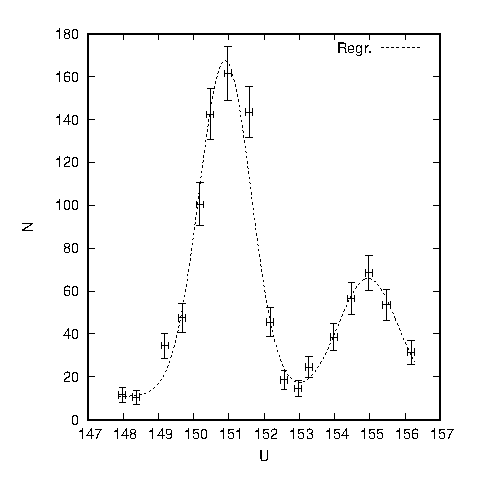
\includegraphics[width=0.7\textwidth]{data/Ba_fein.eps}
  \caption{Aufgezeichnetes Emissionsspektrum von Barium in Feinmessung}
  \label{fig:ba_fein}
\end{figure}
